% TODO: subsection footer
\maketitle

Pesan-pesan error adalah pesan yang ditampilkan di antarmuka (GUI,
TUI, CLI, dll) sebuah perangkat lunak yang akan dibaca oleh pengguna
akhir. Terdapat berbagai pedoman yang dapat digunakan oleh seorang
desainer antarmuka untuk menjaga kualitas antarmuka yang baik.

Satu pedoman karakteristik pesan error yang baik adalah pesan yang:
\begin{pros}
\item Memberikan solusi/langkah berikutnya yang dapat dilakukan oleh
  pengguna secara spesifik (e.g. \texttt{Silahkan muat ulang halaman ini})
\item Berpenampilan sesuai konteks (e.g. penggunaan warna merah)
\item Menggunakan preferensi bahasa pengguna (lokalisasi)
\end{pros}
Sedangkan, pesan error yang buruk memiliki biasanya berupa pesan yang:
\begin{cons}
\item Terlalu generik (e.g. \texttt{SYNTAX ERROR})
\item Tidak dapat dipahami pengguna (e.g. menggunakan kode status
  seperti \texttt{SIGSEGV})
\item Menyalahkan pengguna (e.g. \texttt{Weak password})
\end{cons}

\section{Beragam Contoh Pesan Error Baik dan Buruk}
\subsection{Contoh-contoh Pesan-pesan Error Buruk}

\begin{figure}[H]
  \centering
  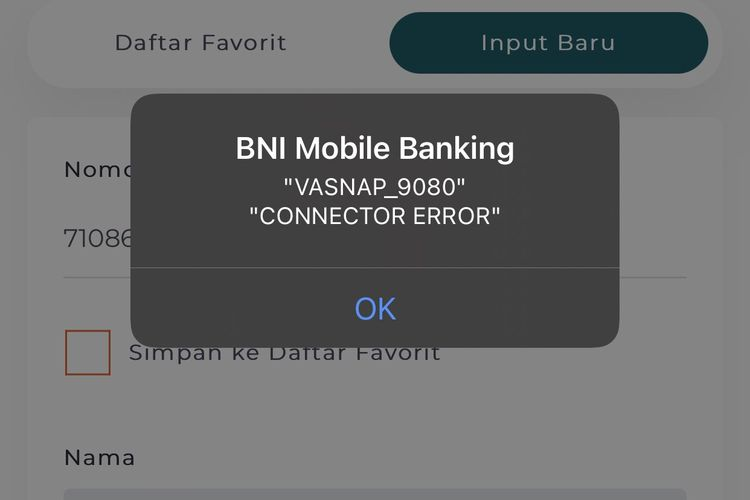
\includegraphics[width=\columnwidth]{bni-bad-1.jpeg}
  \caption{Dialog error pada aplikasi perbankan BNI Mobile Banking}
  \label{fig:bad-err1}
\end{figure}
Gambar \ref{fig:bad-err1} menunjukkan pesan error dengan
karakteristik-karakteristik buruk sebagai berikut:
\begin{cons}
\item Menggunakan kode status \texttt{VASNAP\_9080} yang merupakan kode
  \textit{enum} atau variabel internal yang tidak dapat
  dibaca/dipahami oleh pengguna.
\item Tidak lolos lokalisasi, dikarenakan pesan "\texttt{CONNECTION
  ERROR}" ditulis dalam bahasa inggris, walaupun pengguna menggunakan
  aplikasi dengan bahasa indonesia (dapat dilihat pada konteks belakang dialog)
\end{cons}

Untuk memperbaiki dialog pesan error ini, desainer antarmuka atau
pengembang perangkat lunak yang bersangkutan dapat:
\begin{pros}
\item Menerjemahkan pesan ke bahasa indonesia
\item Memberikan arti dari kode status yang dapat dipahami oleh pengguna
\item Memberikan solusi atau langkah selanjutnya yang dapat dilakukan
  oleh pengguna (e.g. \texttt{Silahkan periksa jaringan anda})
\end{pros}

\begin{figure}[H]
  \centering
  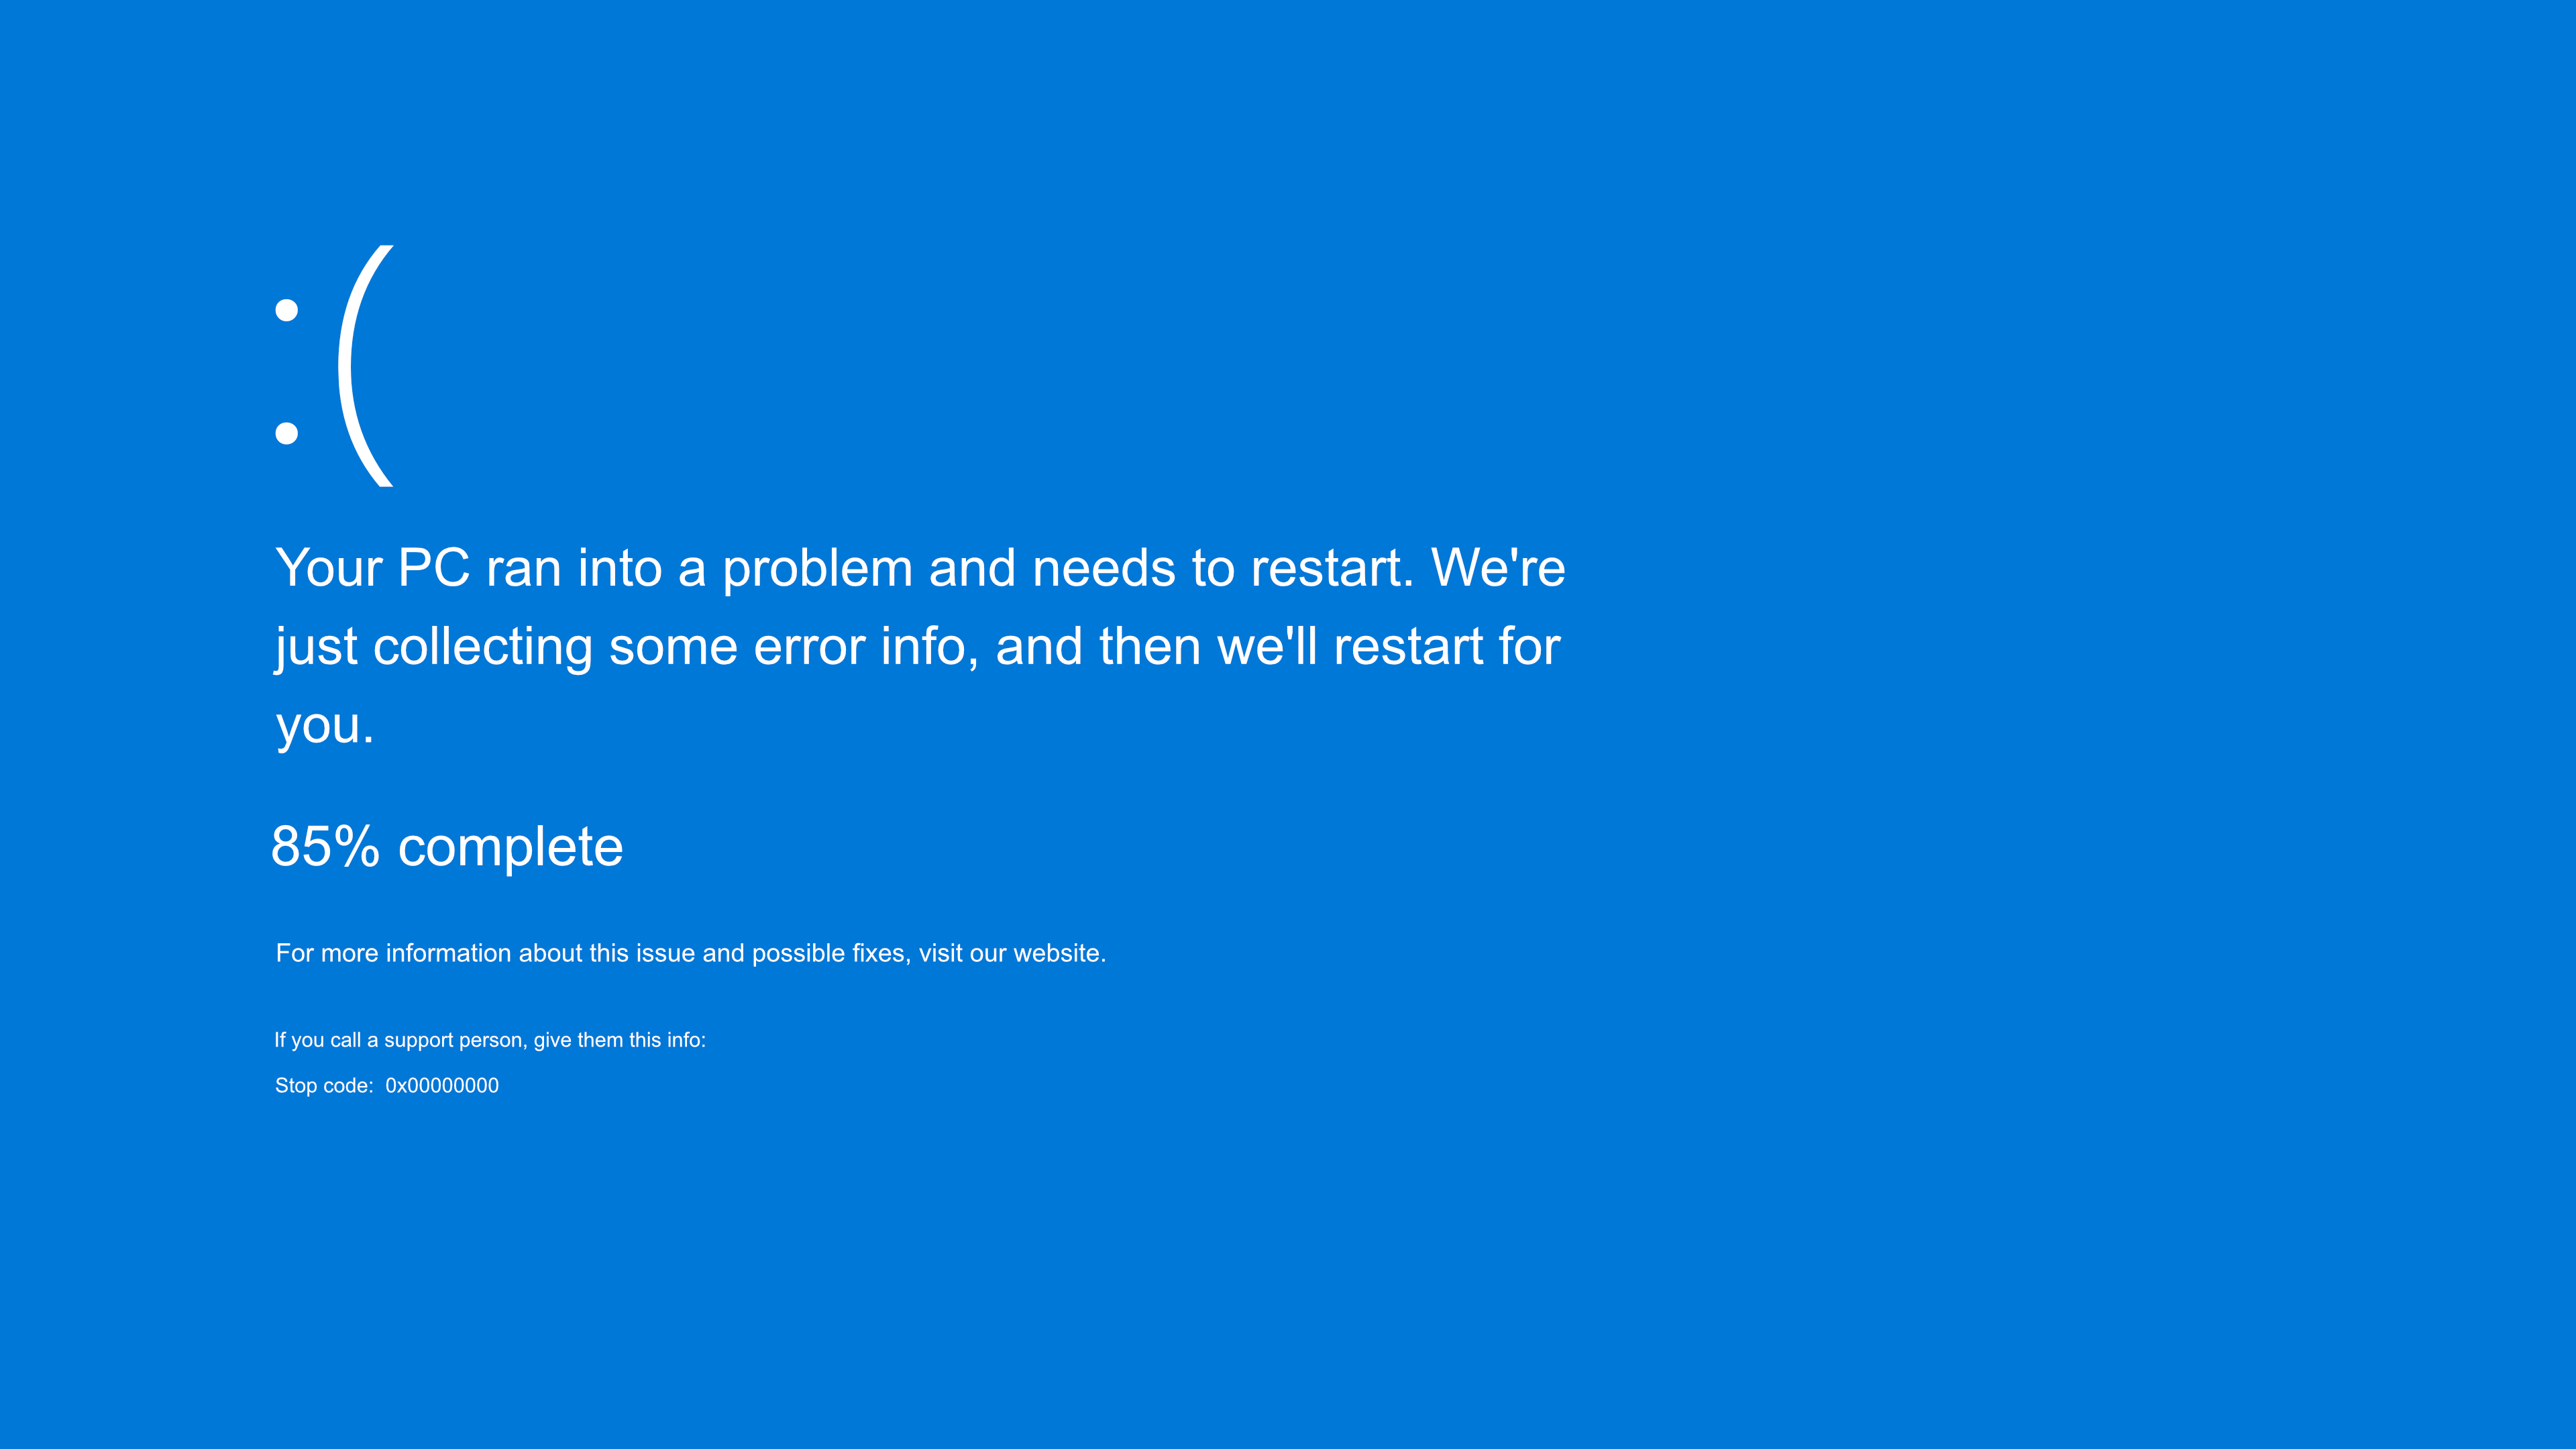
\includegraphics[width=\columnwidth]{bsod-bad.jpg}
  \caption{\textit{Blue Screen Of Death} (BSOD) yang umum ditampilkan pada
    sistem operasi Windows saat terjadi kegagalan sistem yang tidak
  dapat dipulihkan}
  \label{fig:bad-err2}
\end{figure}
BSOD pada gambar \ref{fig:bad-err2} memiliki
karakteristik-karakteristik desain pesan error yang buruk yaitu:
\begin{cons}
\item Menggunakan kode status atau \textit{stop code} yang tidak
  dapat dimengerti oleh pengguna akhir tampa melihat dokumentasi/referensi.
\item Solusi atau langkah yang diberikan kurang spesifik.
  "\textit{Please visit our website}" tidak memberikan alamat
  spesifik yang dapat dikunjungi oleh pengguna.
\end{cons}
Microsoft telah memperbarui tampilan pesan error BSOD versi-versi
Windows terkini (lihat gambar \ref{fig:good-err2}).

\begin{figure}[H]
  \centering
  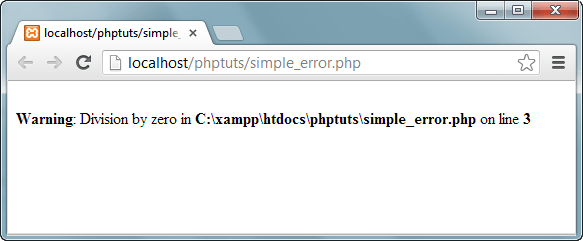
\includegraphics[width=\columnwidth]{php-bad.png}
  \caption{Pesan error PHP yang disengajakan sebagai contoh}
  \label{fig:bad-err3}
\end{figure}
Pada gambar \ref{fig:bad-err3}, terdapat sebuah pesan error dimana
referensi sumber kode disertai dengan nomor baris dimana error atau
kegagalan terjadi ditampilkan. Sifat kerincian pesan error ini
dikarenakan pesan error yang ditampilkan merupakan pesan error yang
ditargetkan kepada pengembang perangkat lunak untuk mendiagnosa
aplikasi. Namun, banyak kasus serupa dimana pengembang menjalankan
aplikasi pada lingkungan produksi tanpa menyetel untuk mematikan
pesan error seperti ini. Sehingga pengguna akhir yang dapat melihat
pesan error yang dapat bersifat sensitif ini.

Dari sudut pedoman desain, pesan error ini memiliki
karakteristik-karakteristik buruk yaitu:
\begin{cons}
\item Tidak dapat dipahami oleh pengguna
\item Tidak memberikan solusi atau langkah berikutnya pada pengguna
\end{cons}
Untuk menangani kasus ini pada lingkungan produksi, pengembang dapat
mengimplementasikan halaman error khusus jika diperlukan dimana pesan
error yang didesain untuk pengguna akhir. Pada lingkungan produksi,
pengembang juga sebaiknya menonaktifkan setelan yang mengaktifkan
penampilan pesan error ini. Biasanya penampilan pesan error ini
disediakan oleh \textit{framework} atau perpustakaan, bahkan bahasa
(seperti PHP) yang digunakan oleh pengembang.

\begin{figure}[H]
  \centering
  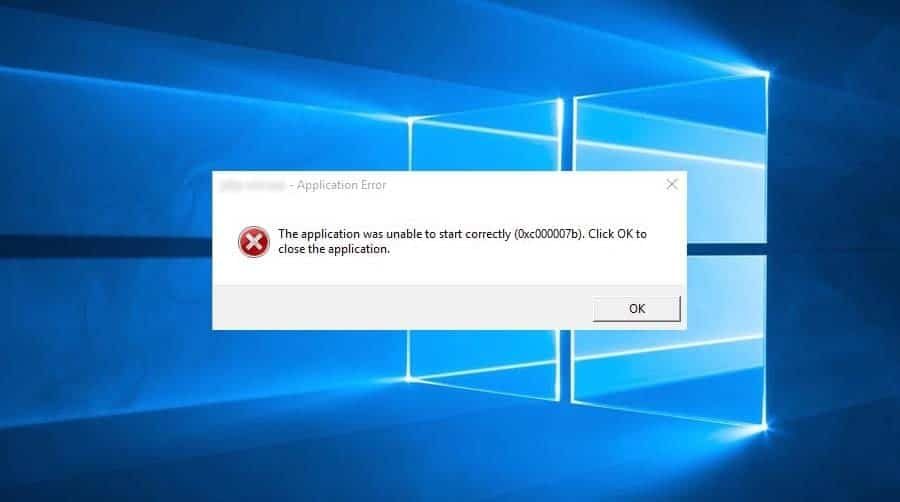
\includegraphics[width=\columnwidth]{generic-windows-bad.jpg}
  \caption{Pesan error umum pada berbagai aplikasi windows}
  \label{fig:bad-err4}
\end{figure}
Di gambar \ref{fig:bad-err4}, serupa dengan pesan pada gambar
\ref{fig:bad-err1}; pesan error tersebut memiliki karakteristik buruk
antara lain:
\begin{cons}
\item Menggunakan kode status \texttt{0xc000007b} yang tidak dapat
  dipahami oleh pengguna.
\item Pesan error yang terlalu generik, alasan mengapa aplikasi tidak
  dapat berjalan tidak diberikan.
\item Tidak memberikan solusi atau langkah selanjutnya pada pengguna.
\end{cons}
Alasan sebenarnya dibalik kasus error ini (menurut
\url{https://stackoverflow.com/a/10493137/24319043}) adalah langkah
eksekusi program 32 bit pada sistem 64 bit, atau sebaliknya. Sehingga
pengembang dapat menambahkan alasan tersebut pada pesan error di atas
untuk memperbaiki pesan tersebut.

\begin{figure}[H]
  \centering
  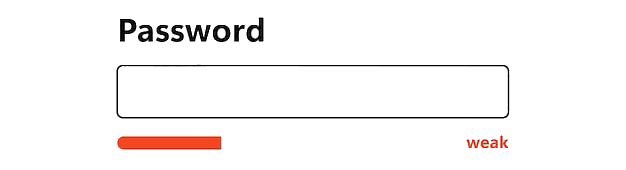
\includegraphics[width=\columnwidth]{password-bad.png}
  \caption{Contoh antarmuka input password yang umum digunakan}
  \label{fig:bad-err5}
\end{figure}
Menurut pedoman di atas, antarmuka pada gambar \ref{fig:bad-err5}
memiliki karakteristik-karakteristik buruk yaitu:
\begin{cons}
\item Pesan terlalu generik, tidak diberikan terkait mengapa password
  yang diberikan baik atau buruk.
\item Menyalahkan pengguna jika password yang diberikan lemah.
\end{cons}
Untuk menanggulangi kasus ini, pengembang dapat
\begin{pros}
\item Menampilkan kriteria-kriteria password yang harus dipenuhi
\item Mengganti ungkapan \texttt{weak} dengan kriteria yang belum
  dipenuhi oleh pengguna
\end{pros}

\begin{figure}[H]
  \centering
  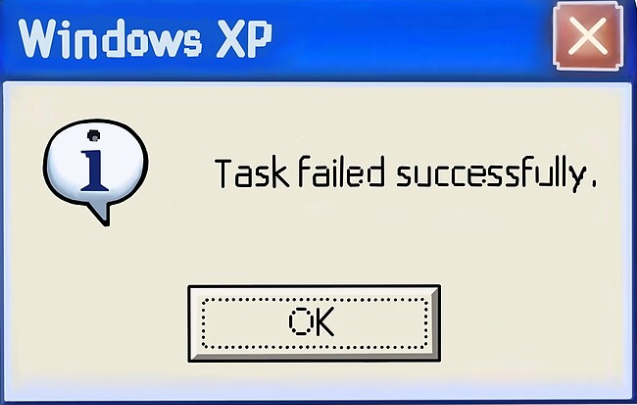
\includegraphics[width=0.5\columnwidth]{bonus-bad.png}
  \caption{Bonus}
\end{figure}

\subsection{Contoh-contoh Pesan-pesan Error Baik}

\begin{figure}[H]
  \centering
  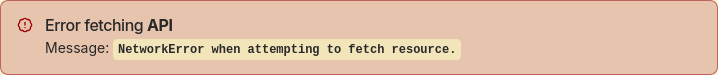
\includegraphics[width=\columnwidth]{phantomports-good.png}
  \caption{Antarmuka dialog pesan error
  \url{https://phantomports.com} saat terjadi kegagalan jaringan}
  \label{fig:good-err1}
\end{figure}
\begin{info}{Catatan Penulis}
  Aplikasi pada gambar \ref{fig:good-err1} merupakan aplikasi pribadi
  yang dengan sumber kode di
  \url{https://github.com/arsmoriendy/phantomports-front}
\end{info}
Pesan error pada gambar \ref{fig:good-err1} memiliki karakteristik
sebagai berikut:
\begin{pros}
\item Tidak menggunakan kode status, pesan dapat dipahami oleh pengguna akhir
\item Memiliki rincian spesifik mengapa kegagalan terjadi, tidak generik
\end{pros}

\begin{figure}[H]
  \centering
  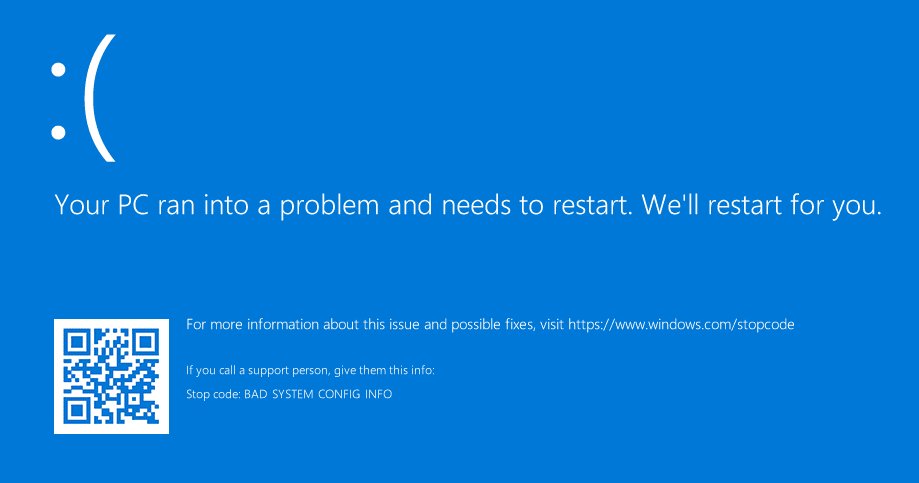
\includegraphics[width=\columnwidth]{bsod-good.png}
  \caption{Contoh pesan BSOD (serupa dengan gambar
  \ref{fig:bad-err2}) pada versi-versi baru sistem operasi Windows}
  \label{fig:good-err2}
\end{figure}
Gambar \ref{fig:good-err2} merupakan perbaikan antarmuka BSOD yang
telah dilakukan oleh Microsoft. Walaupun tidak sempurna, versi BSOD
ini memiliki:
\begin{pros}
\item Kode QR yang dapat mengalihkan pengguna ke sumber referensi
  error yang dapat dipahami
\item Kode error "\texttt{BAD SYSTEM CONFIG INFO}" yang lebih spesifik
\item Alamat situs web dokumentasi error di
  "\url{https://www.windows.com/stopcode}"
\end{pros}

\begin{figure}[H]
  \centering
  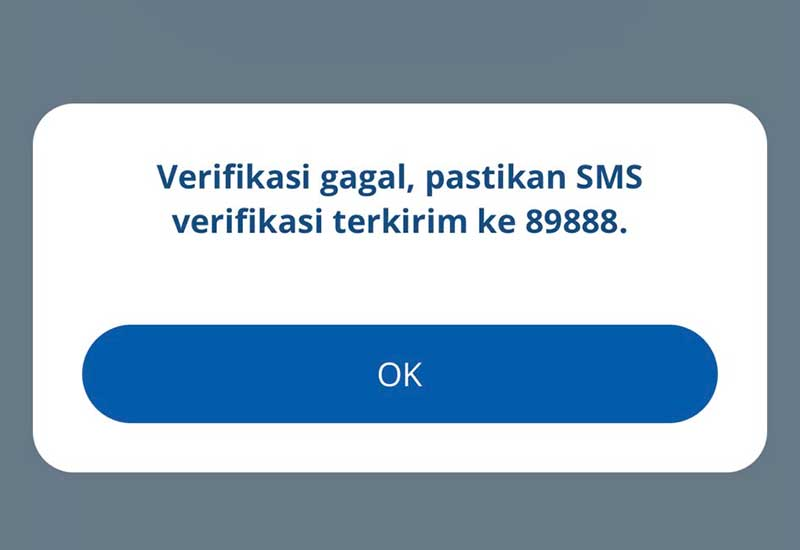
\includegraphics[width=\columnwidth]{bca-good.jpg}
  \caption{Pesan error saat pembuatan akun pada aplikasi MyBCA}
  \label{fig:good-err3}
\end{figure}
Pesan di gambar \ref{fig:good-err3} memiliki karakteristik-karakteristik:
\begin{pros}
\item Memberi pengguna langkah selanjutnya untuk menanggulangi
  kegagalan yang dihadapi
\item Lokalisasi pesan menggunakan bahasa indonesia
\end{pros}

\begin{figure}[H]
  \centering
  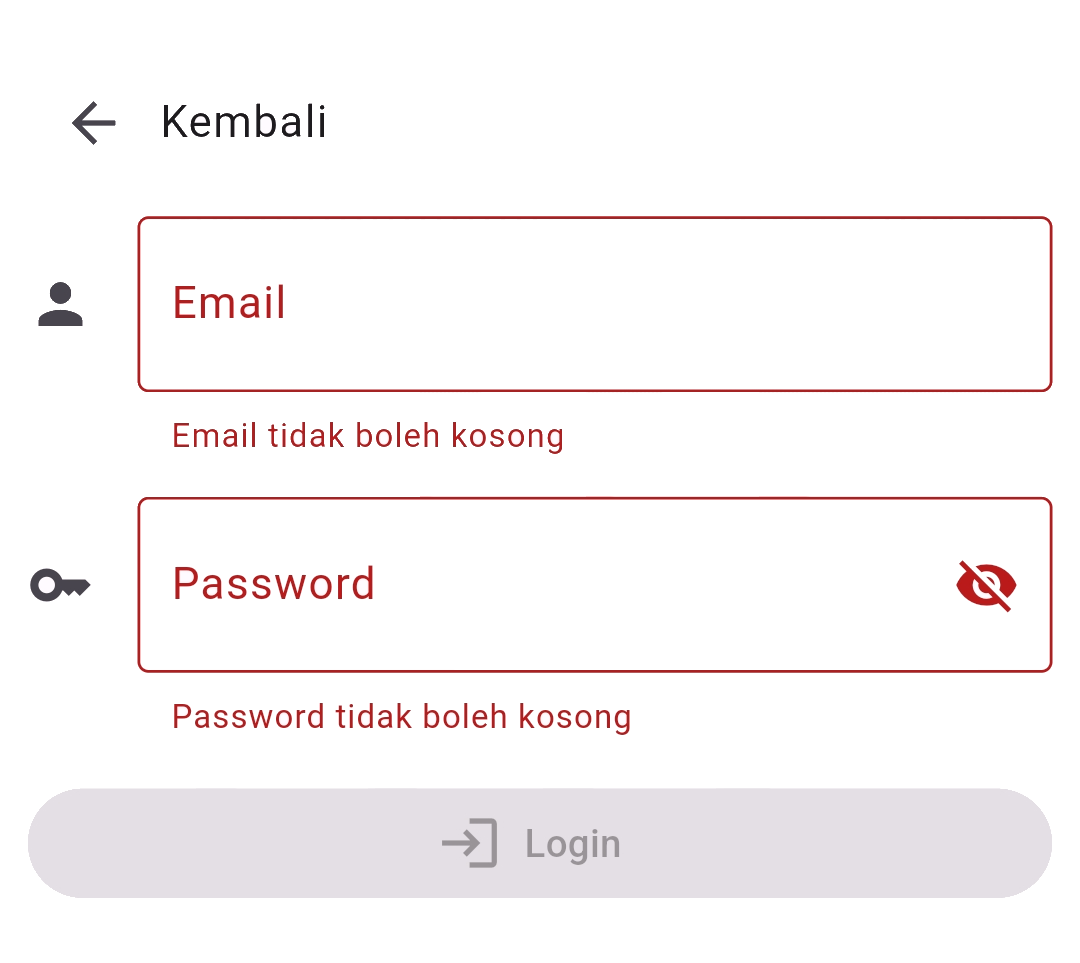
\includegraphics[width=\columnwidth]{pt-good.png}
  \caption{Pesan error yang mengindikasikan bahwa kriteria input
  belum terpenuhi dari aplikasi Pejuang Tani}
  \label{fig:good-err4}
\end{figure}
\begin{info}{Catatan Penulis}
  Aplikasi pada gambar \ref{fig:good-err4} merupakan aplikasi pribadi
  yang disimpan di:
  \begin{itemize}
    \item \url{https://github.com/stnDinus/uas_ppb_server} (server, public)
    \item \url{https://github.com/stnDinus/uas_ppb} (client, private)
  \end{itemize}
\end{info}
Pada gambar \ref{fig:good-err4}, pesan-pesan error memiliki ciri-ciri:
\begin{pros}
\item Dapat dipahami oleh pengguna, tidak menggunakan kode status
\item Menggunakan saran objektif, tanpa menyalahkan pengguna
\item Warna konteks yang familiar, yaitu tombol \textit{Login}
  berwarna abu-abu yang mengindikasikan tidak dapat diketuk, teks
  error berwarna merah.
\end{pros}

\begin{figure}[H]
  \centering
  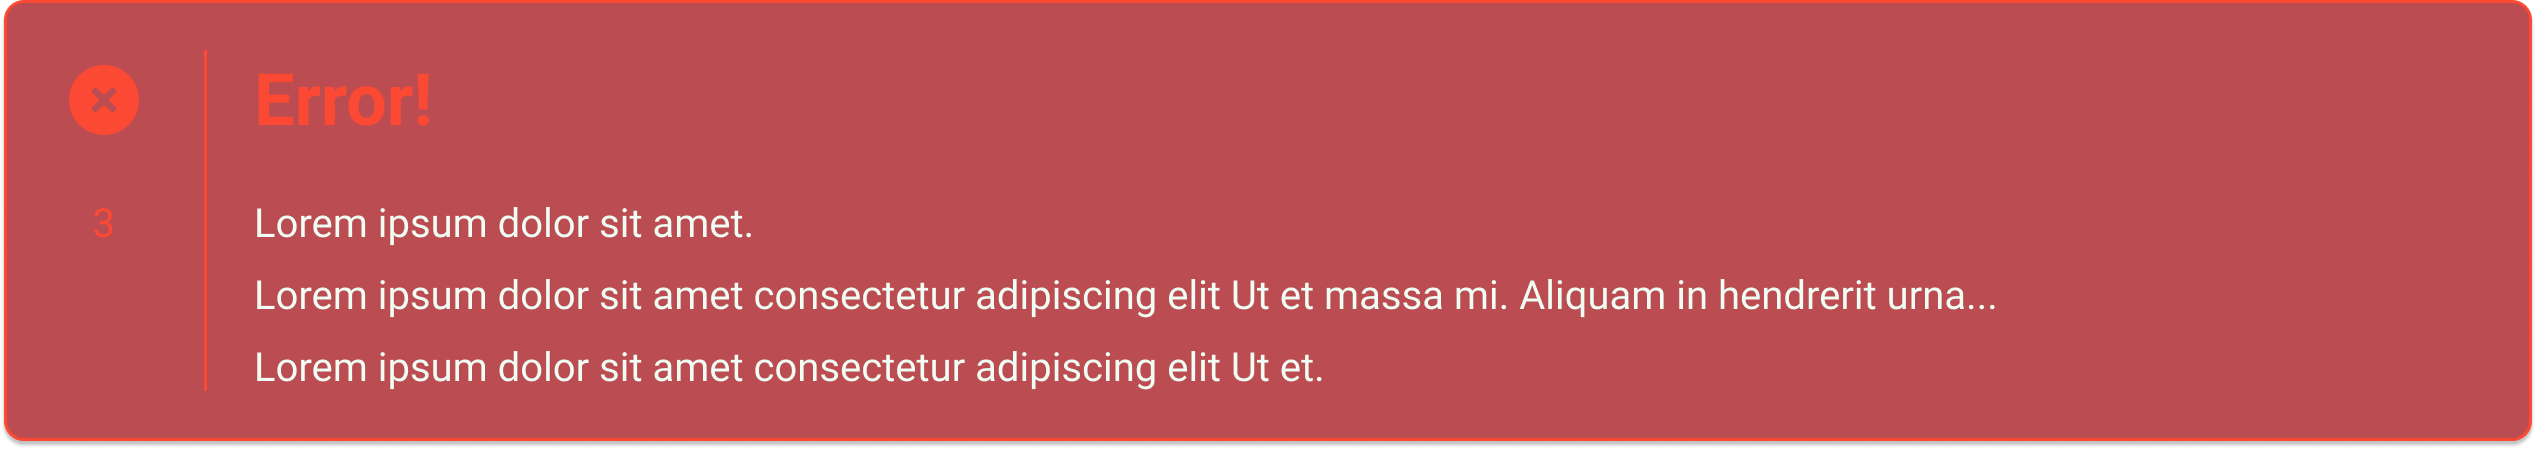
\includegraphics[width=\columnwidth]{concept-good.png}
  \caption{Konsep dialog error}
  \label{fig:good-err5}
\end{figure}
\begin{info}{Catatan Penulis}
  Konsep pada gambar \ref{fig:good-err5} merupakan desain pribadi
  yang dapat dilihat di
  \url{https://www.figma.com/design/Lox4KX1iKN2ZUHeweQrpc7/Alerts?node-id=0-1&t=yltzRAXqFTp7kYVg-1}
\end{info}
Pesan error pada gambar \ref{fig:good-err5} memiliki ciri-ciri:
\begin{pros}
\item Warna merah dengan icon silang yang memberi konteks error yang jelas
\item Menganjurkan pengembang dari desain untuk tidak menggunakan
  kode status, dengan \textit{placeholder} teks yang rinci
\end{pros}
